\documentclass{beamer}
\usepackage[T1]{fontenc}
\usepackage[utf8]{inputenc}
\usepackage[UKenglish]{babel}
\usepackage{booktabs}
\usepackage{graphicx}

\usetheme{default}
\setbeamertemplate{footline}[frame number]
\title{EIST -- T02 Team Project}
\subtitle{Flight System GAFIS}
\author{Scrumbags}
\institute{Technische Universität München}
\date{29 July 2022}
%
\begin{document}
\begin{frame}[plain]
\titlepage
\end{frame}
%
\begin{frame}{Outline}
\tableofcontents
\end{frame}

\AtBeginSubsection[ ] {
	\begin{frame}{Outline}
		\tableofcontents[currentsection,currentsubsection]
	\end{frame}
	\addtocounter{framenumber}{-1}
}

\AtBeginSection[ ] {
	\begin{frame}{Outline}
		\tableofcontents[currentsection]
	\end{frame}
	\addtocounter{framenumber}{-1}
}
\section{Problem Statement}
\begin{frame}{Flight System}
	Design a system to make traveling via airplane more pleasant
	\begin{itemize}
		\item Get Information about the current flight
		\item Get points of interest at destination
		\item Create flight journeys
		\item Enjoy movies, food and drinks
		\item \dots
	\end{itemize}
\end{frame}
\section{High-Level Objectives}
\subsection{Back-End}
\begin{frame}{Weather, Movies, Flights, Maps, POIs}
	Fetch and present data from external services
	\begin{figure}
		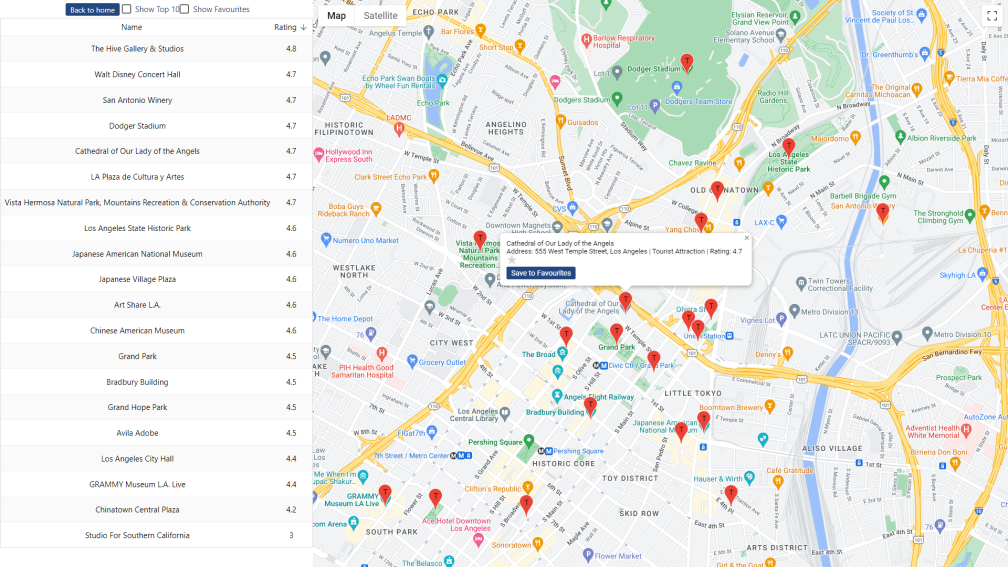
\includegraphics[width=.8\textwidth]{../images/AboutMyDestination.png}
		\caption{Points of interest at destination}
	\end{figure}
\end{frame}

\begin{frame}{Flight information and Survey}
	Create a login system
	\begin{itemize}
		\item Extend system functionality if logged in
		\item Grant persistance of information
	\end{itemize}
	\begin{figure}
		\includegraphics[width=0.7\textwidth]{../images/survey.png}
		\caption{Logged-in users can take a survey}
	\end{figure}
\end{frame}
%
\subsection{Front-End}
\begin{frame}{UI}
	Intuitive to use and easy to understand
	\begin{itemize}
		\item Complete all interactions in $< 3$ clicks
	\end{itemize}
\end{frame}
%
\section{Functional Requirements}
\subsection{Flights}
\begin{frame}{Flights}
	\begin{itemize}
		\item Show flight information and get notified about changes
		\item Build flight trips from hand-picked flights
		\item Display destination information
	\end{itemize}
	\begin{figure}
		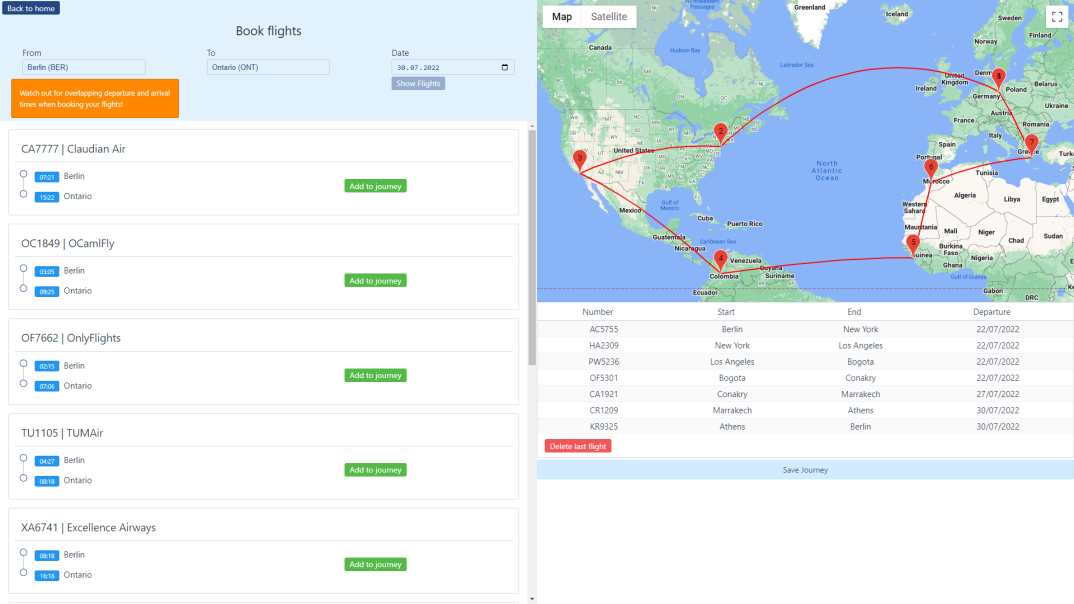
\includegraphics[width=.8\textwidth]{../images/BookFlights.png}
		\caption{Build flight journeys}
	\end{figure}
\end{frame}
%
\subsection{Logged-in Functionality}
\begin{frame}{Feedback}
	\begin{itemize}
		\item Take survey on flight comfort, catering, \dots
	\end{itemize}
	\begin{figure}
		\includegraphics[width=0.8\textwidth]{../images/survey.png}
		\caption{Logged-in users can take a survey}
	\end{figure}
\end{frame}
%
\subsection{General Functionality}
\begin{frame}{Infotainment}
	\begin{itemize}
		\item Watch movies and order food and drinks
		\item Request assistance
		\item Watch flight safety instructions
	\end{itemize}
	\begin{figure}
		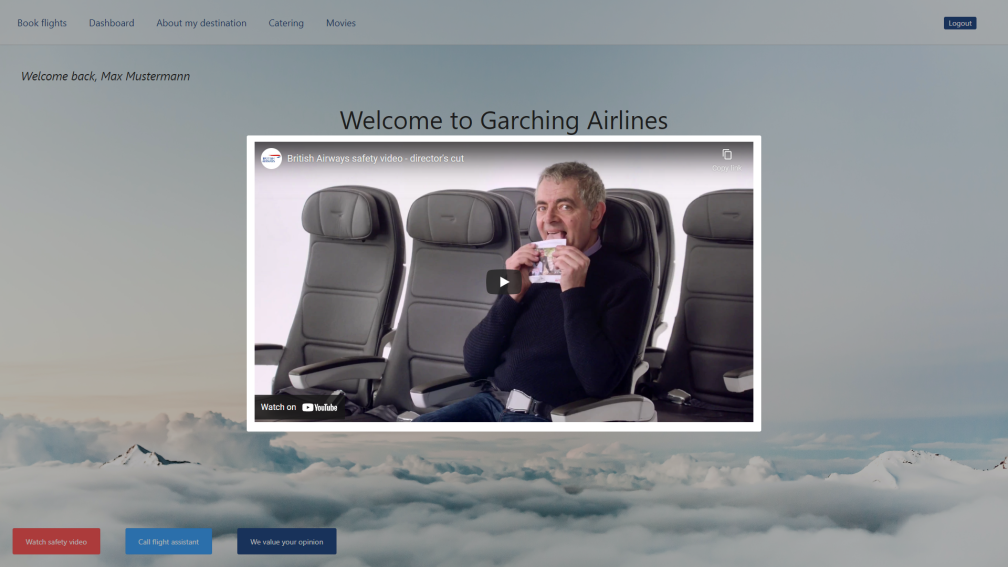
\includegraphics[width=.8\textwidth]{../images/SafetyVideo.png}
		\caption{Safety video}
	\end{figure}
\end{frame}
\section{System Design}
\subsection{Analysis Object Model}
\begin{frame}{\href{run:../images/ObjectDiagram.png}{Analysis Object Model}}
	\begin{figure}
		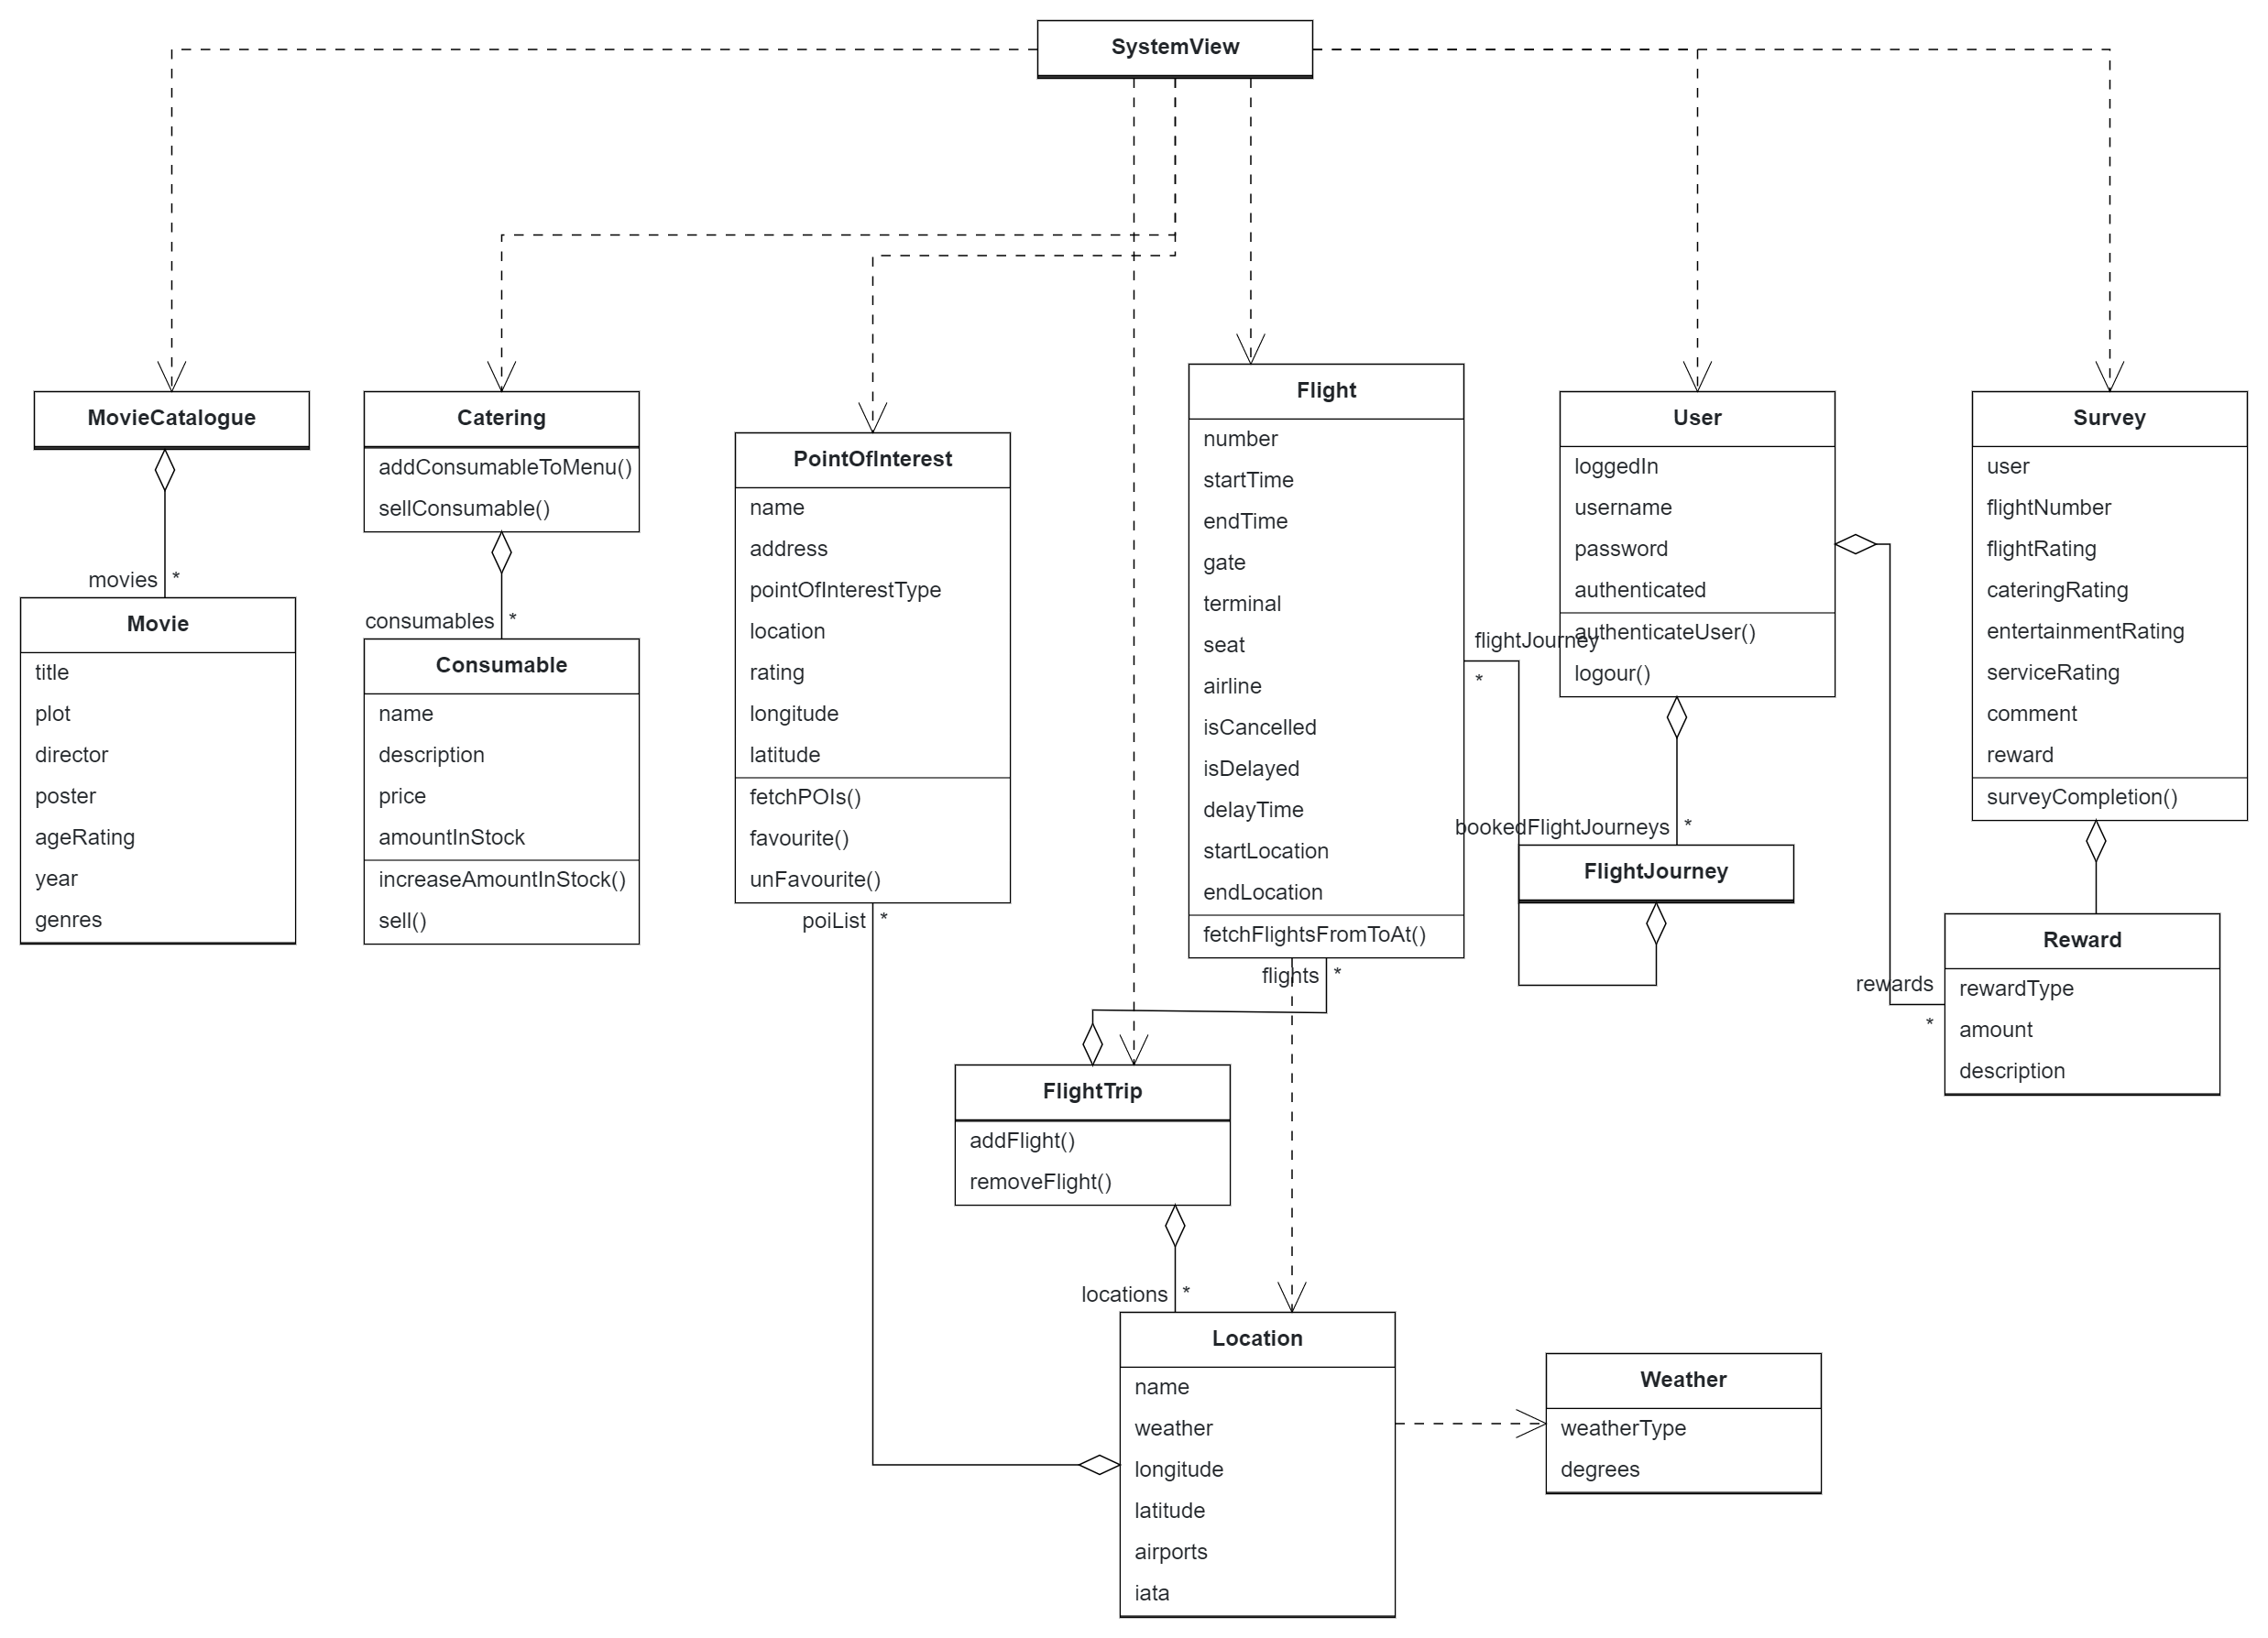
\includegraphics[width=.8\textwidth]{../images/ObjectDiagram.png}
	\end{figure}
\end{frame}
\subsection{Top Level Design}
\begin{frame}{\href{run:../images/SubsystemDecomposition.PNG}{Subsystem Decomposition}}
	\begin{figure}
		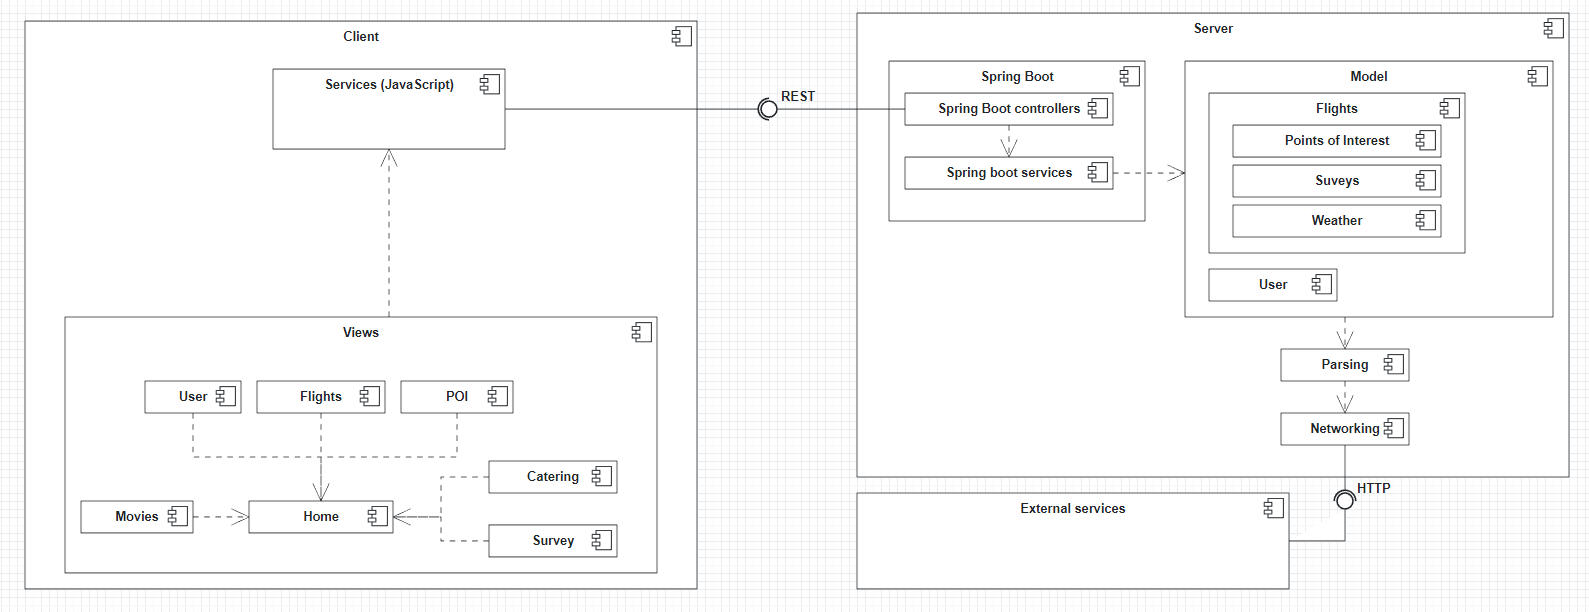
\includegraphics[width=\textwidth]{../images/SubsystemDecomposition.PNG}
	\end{figure}
\end{frame}
\subsection{Communication Model}
\begin{frame}{\href{run:../images/ScenarioOneCommunication.png}{Communication Model}}
	\begin{figure}
		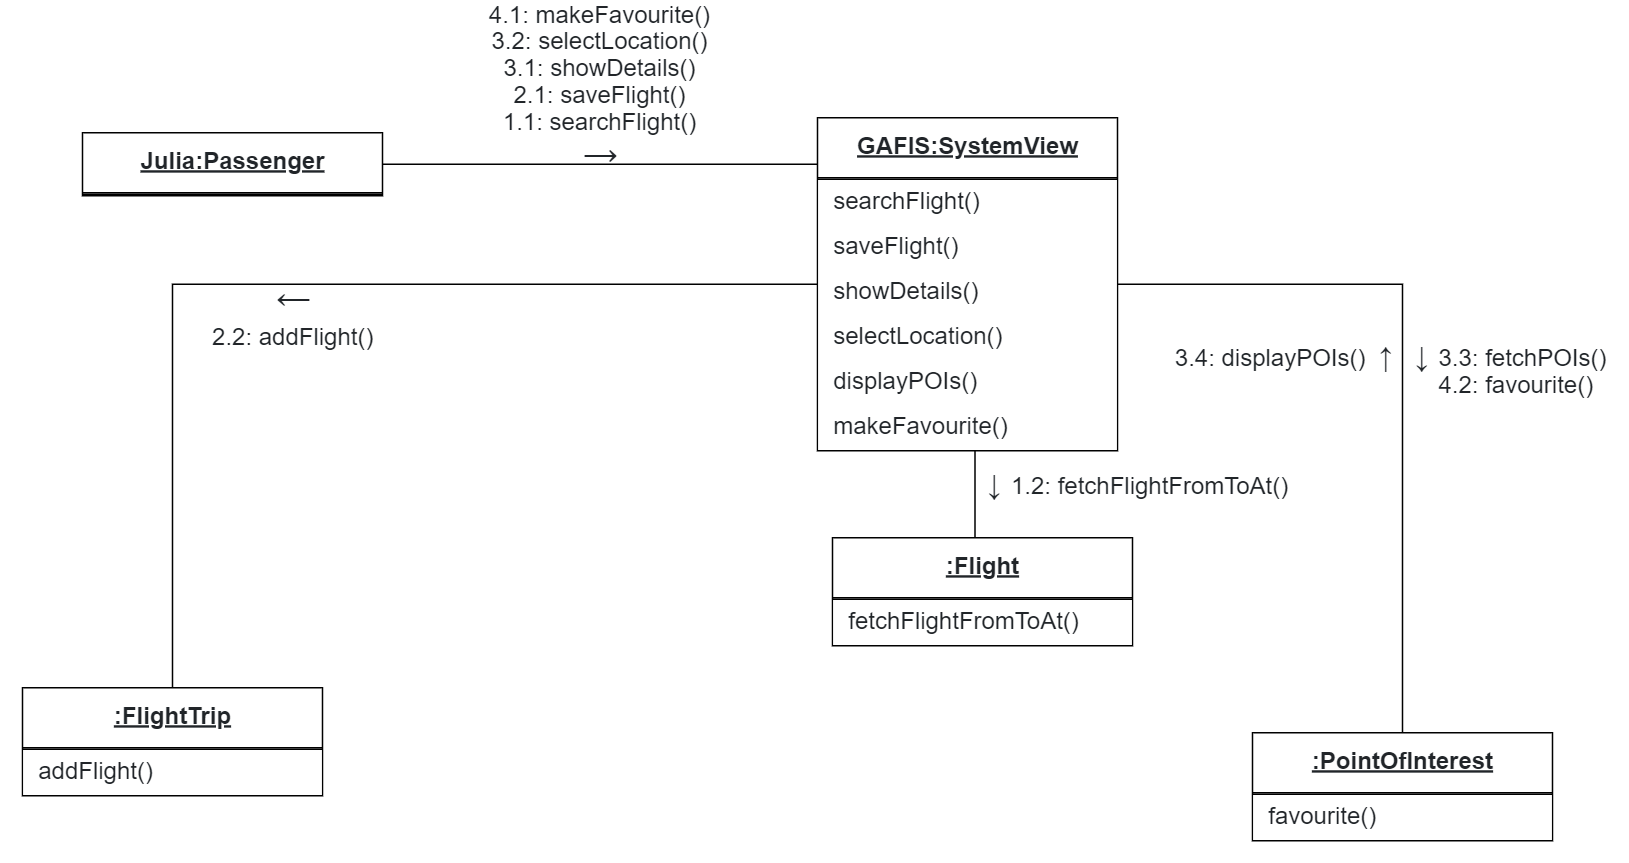
\includegraphics[width=.8\textwidth]{../images/ScenarioOneCommunication.png}
		\caption{Julia's flight from Munich to Lisbon}
	\end{figure}
\end{frame}
\section{Demonstration}
\section{Current Status and Future Work}
\end{document}
